\chapter{RL-Based Adaptive Image-Text Fusion Approach}


\section{Introduction}


This chapter presents the conceptual approach proposed in this research. The purpose of the approach is to extend multimodal fake news detection by replacing a fixed image-text fusion rule with an adaptive and explainable fusion policy. The approach treats fusion as an action-selection problem in which a reinforcement learning controller observes reliability-related features and selects how much influence should be assigned to the image and text branches.


\section{Hypothesis and Inspiration}


The hypothesis of this research is that a reliability-aware adaptive fusion policy can provide competitive fake news detection performance while making the modality contribution more explainable at sample level. The approach is inspired by the observation that image and text evidence are not equally reliable for every social media post. A fixed fusion method applies the same rule even when one modality is uncertain, noisy, or in conflict with the other modality. An adaptive policy can instead select a fusion action based on the observed reliability state of the sample.


\section{Inputs and Outputs of the Proposed Extension}


The inputs to the proposed extension are the outputs of the image and text branches, together with reliability indicators derived from the sample. The image branch produces an image probability and an image confidence value. The text branch produces a text probability and a text confidence value. Additional reliability indicators represent image quality, text quality, modality disagreement, confidence difference, and quality difference.


The main output is a binary fake news prediction using the label standard 0 for real and 1 for fake. The framework also outputs the final probability, selected fusion action, image weight, text weight, and explanation artifacts. These outputs make the decision more inspectable than a prediction label alone.


\section{Process Workflow of the Proposed Extension}


The proposed workflow contains six conceptual stages, as illustrated in Figure 4.1. First, the dataset is prepared and labels are standardized. Second, the image and text branches are trained separately. Third, both branches generate prediction probabilities for each split. Fourth, reliability features are computed and merged with modality predictions. Fifth, the reinforcement learning fusion controller selects a fusion action for each sample. Sixth, the framework generates classification metrics, policy analysis, robustness results, and explanation outputs.


The process is designed to separate unimodal representation learning from adaptive decision fusion. This separation allows the fusion controller to remain lightweight, because it uses a compact reliability-aware state instead of processing raw images or raw text directly.


The methodological contribution is the replacement of a fixed post-hoc fusion rule with a sample-level controller that observes reliability evidence before assigning modality weights. The novelty comparison diagram in this chapter makes this distinction explicit by separating simple fixed fusion from the proposed reliability-aware action-selection path.


\section{Reliability-Aware State Representation}


The reliability-aware state is the main input to the fusion controller. It contains:


1. Image prediction probability.

2. Image confidence.

3. Image quality.

4. Text prediction probability.

5. Text confidence.

6. Text quality.

7. Modality disagreement.

8. Confidence difference.

9. Quality difference.


This state representation was selected to capture both branch-level prediction strength and cross-modal conflict. The image and text probabilities represent the direct unimodal evidence. The confidence features represent prediction certainty. The quality features provide engineered reliability cues. Disagreement and difference features help the controller identify samples where the modalities may require more careful balancing.


\section{Adaptive Fusion Action Space}


The reinforcement learning controller selects from a discrete set of fusion actions. Each action maps to a fixed pair of image and text weights. This design makes the policy easy to interpret because each selected action can be directly translated into a modality trust decision. A continuous action space may provide finer control, but the discrete action space was selected for simplicity, stability, and explainability.


\section{Reward Design}


The reward is based on whether the fused prediction is correct. If the selected fusion action leads to a correct prediction, the controller receives a positive reward. If the prediction is incorrect, it receives a negative reward. This binary reward directly connects the policy to classification correctness.


The reward design is intentionally simple. It supports clear interpretation but does not distinguish between highly confident and marginally correct predictions. A margin-based or log-loss-based reward is therefore identified as a possible future improvement.


\section{Explanation Strategy}


The framework provides transparent decision evidence at three levels. At the image level, Grad-CAM heatmaps highlight visual regions associated with the image prediction. At the text level, token saliency identifies influential tokens from the text branch. At the fusion level, the selected action, image weight, text weight, final probability, and final prediction show how the modalities were combined.


This transparency strategy is aligned with the research problem because it does not stop at model performance. It provides inspectable decision evidence about the modality weighting process without claiming a complete causal explanation of the final prediction.


\section{Positioning within the AI Body of Knowledge}


The proposed extension lies at the intersection of multimodal learning, reinforcement learning, and explainable AI. The image and text branches provide unimodal deep learning representations. The fusion controller applies reinforcement learning to select a decision action based on a compact state. The explanation layer supports interpretability by exposing modality weights and branch-level saliency.


The contribution is not the invention of a new image encoder or language model. Instead, the contribution is a reliability-aware contextual-bandit-style reinforcement learning controller that makes image-text fusion adaptive, inspectable, and reproducible for fake news detection.


\section{Summary}


This chapter presented the proposed RL-based adaptive image-text fusion approach. The approach uses separate image and text branches, a reliability-aware state representation, a discrete fusion action space, and explanation outputs. The next chapter converts this conceptual approach into a system-level analysis and design.

The image and text branches are represented by functions that output fake-class probabilities:

\begin{equation}
p_i = f_i(x_i), \qquad p_t = f_t(x_t)
\label{eq:unimodal_probabilities}
\end{equation}

The confidence of each modality is computed from the stronger binary-class probability:

\begin{equation}
c_m = \max(p_m, 1-p_m), \qquad m \in \{i,t\}
\label{eq:modality_confidence}
\end{equation}

The reliability-aware state used by the fusion controller is defined as:

\begin{equation}
s = [p_i, c_i, q_i, p_t, c_t, q_t, |p_i-p_t|, c_i-c_t, q_i-q_t]
\label{eq:reliability_state}
\end{equation}

\begin{figure}[htbp]
\centering
\resizebox{\textwidth}{!}{%
\begin{tikzpicture}[
    node distance=1.3cm and 1.5cm,
    block/.style={
        rectangle,
        rounded corners,
        draw=black,
        thick,
        align=center,
        minimum width=3.4cm,
        minimum height=1.0cm,
        fill=blue!7
    },
    model/.style={
        rectangle,
        rounded corners,
        draw=black,
        thick,
        align=center,
        minimum width=3.6cm,
        minimum height=1.0cm,
        fill=green!10
    },
    fusion/.style={
        rectangle,
        rounded corners,
        draw=black,
        thick,
        align=center,
        minimum width=4.0cm,
        minimum height=1.1cm,
        fill=orange!15
    },
    output/.style={
        rectangle,
        rounded corners,
        draw=black,
        thick,
        align=center,
        minimum width=3.6cm,
        minimum height=1.0cm,
        fill=purple!10
    },
    eval/.style={
        rectangle,
        rounded corners,
        draw=black,
        thick,
        align=center,
        minimum width=3.8cm,
        minimum height=1.0cm,
        fill=gray!12
    },
    arrow/.style={->, thick}
]

% Data layer
\node[block] (data) {Fakeddit Multimodal Dataset\\Image--Text Posts};
\node[block, below=of data] (prep) {Data Preparation\\Label Standardization\\Train/Validation/Test Splits};

% Modality branches
\node[model, below left=1.4cm and 1.9cm of prep] (image) {Image Branch\\ResNet-18 Fine-Tuning\\Image Probability + Confidence};
\node[model, below right=1.4cm and 1.9cm of prep] (text) {Text Branch\\DistilBERT Fine-Tuning\\Text Probability + Confidence};

% Reliability
\node[block, below=2.0cm of prep] (reliability) {Reliability Feature Extraction\\Image Quality, Text Quality\\Disagreement, Confidence Difference};

% State and fusion
\node[fusion, below=of reliability] (state) {9-Dimensional Reliability State\\Probabilities + Confidence + Quality + Disagreement};
\node[fusion, below=of state] (rl) {RL-Based Adaptive Fusion Controller\\Contextual Action Selection\\Fusion Weights $(w_i, w_t)$};
\node[output, below=of rl] (pred) {Final Fake News Prediction\\Fused Probability\\Real/Fake Label};

% Explainability
\node[output, left=1.8cm of pred] (explain) {Explainability Outputs\\Grad-CAM Heatmaps\\Token Saliency\\Fusion Weights};

% Evaluation
\node[eval, right=1.8cm of pred] (evals) {Evaluation\\Baselines, MLP, Controllers\\Ablation, Robustness\\McNemar + Seed Tests};

% Arrows
\draw[arrow] (data) -- (prep);
\draw[arrow] (prep) -- (image);
\draw[arrow] (prep) -- (text);
\draw[arrow] (image) -- (reliability);
\draw[arrow] (text) -- (reliability);
\draw[arrow] (reliability) -- (state);
\draw[arrow] (state) -- (rl);
\draw[arrow] (rl) -- (pred);
\draw[arrow] (image) |- (explain);
\draw[arrow] (text) |- (explain);
\draw[arrow] (rl) -- (explain);
\draw[arrow] (pred) -- (evals);
\draw[arrow] (rl) -- (evals);

% Baseline comparison note
\node[eval, below=0.9cm of evals] (baselines) {Comparison Methods\\Equal Fusion\\Confidence/ Reliability Fusion\\Logistic Regression\\Decision Trees\\Supervised MLP};
\draw[arrow] (evals) -- (baselines);

\end{tikzpicture}%
}
\caption{Overall architecture of the proposed explainable reinforcement learning-based adaptive image-text fusion framework for fake news detection.}
\label{fig:proposed_architecture}
\end{figure}

\begin{figure}[H]
\centering
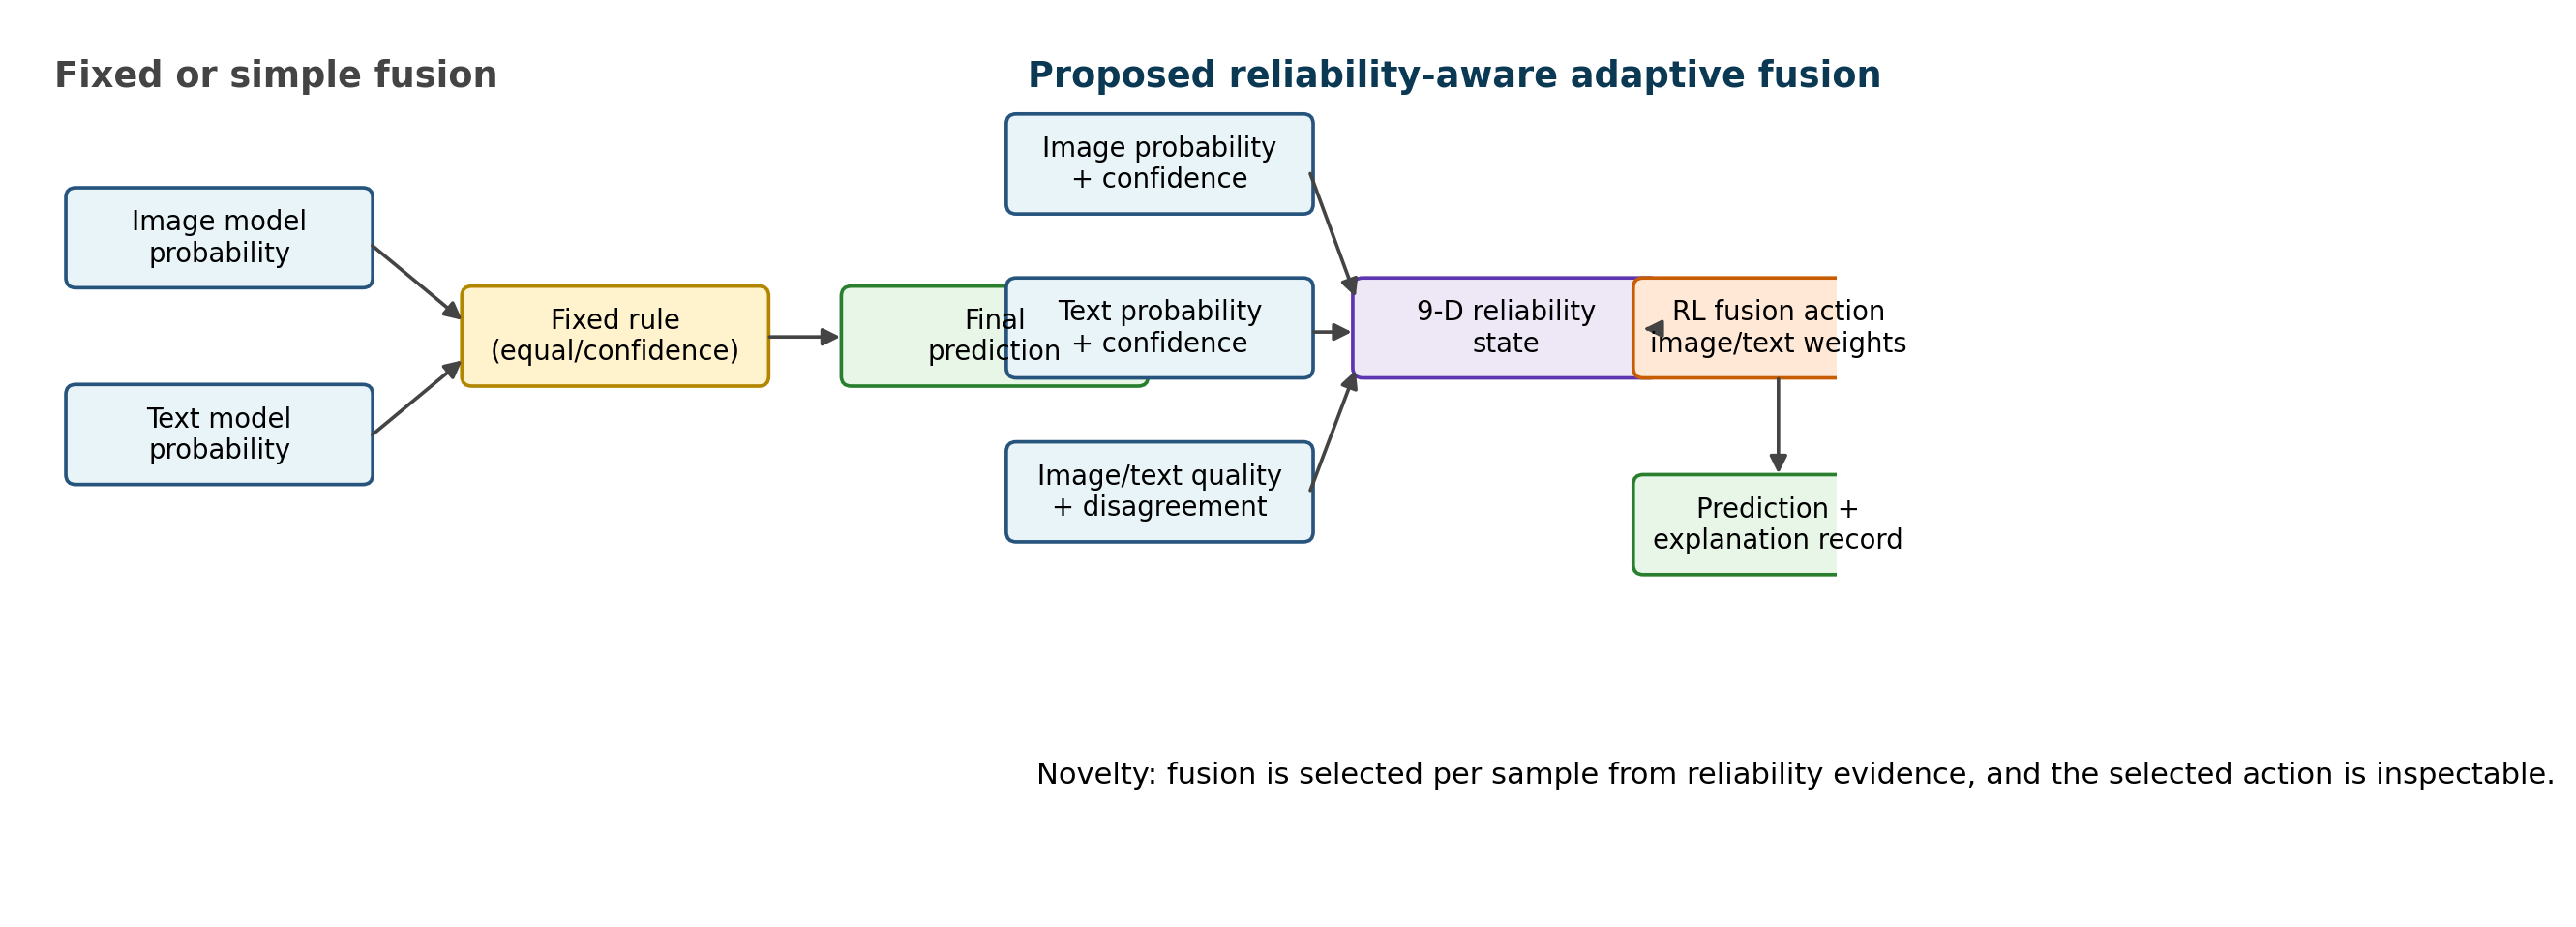
\includegraphics[width=0.92\textwidth,height=0.42\textheight,keepaspectratio]{figures/figure_4_2_novelty_architecture_difference.png}
\caption{Structural difference between fixed fusion and the proposed reliability-aware adaptive fusion controller.}
\label{fig:novelty_architecture_difference}
\end{figure}

Each discrete action maps to an interpretable image-text weighting pair:

\begin{equation}
\begin{aligned}\mathcal{A}=\{&(0.90,0.10),(0.75,0.25),(0.60,0.40),(0.50,0.50),\\ &(0.40,0.60),(0.25,0.75),(0.10,0.90)\}\end{aligned}
\label{eq:action_space}
\end{equation}

\begin{equation}
a_k \mapsto (w_i^{(k)}, w_t^{(k)}), \qquad w_i^{(k)} + w_t^{(k)} = 1
\label{eq:action_weight_mapping}
\end{equation}

The final fake-class probability is then produced by weighted late fusion:

\begin{equation}
p_f = w_i^{(k)}p_i + w_t^{(k)}p_t
\label{eq:fused_probability}
\end{equation}

The binary decision rule is:

\begin{equation}
\hat{y}=\begin{cases}1, & p_f \ge \tau \\ 0, & p_f < \tau\end{cases}
\label{eq:prediction_rule}
\end{equation}

The reward function links the selected fusion action directly to classification correctness:

\begin{equation}
r(s,a_k)=\begin{cases}+1, & \hat{y}=y \\ -1, & \hat{y}\ne y\end{cases}
\label{eq:reward_function}
\end{equation}

\clearpage
